%!TEX root = ../Thesis.tex
%!TEX program = xelatex
\documentclass[../Thesis]{subfiles}

% 本文
\begin{document}
\chapter{はじめに}
\label{cha:はじめに}
\section{背景}
  近年、豪雨による斜面崩壊・浸水被害が多発しており、災害の危険性が高まる1時間降水量50mm以上の大雨は統計期間最初の10年間(1976~1985年)に比べ最近10年間(2011~2020年)での平均年間発生回数は約1.4倍に増加している\cite{web01}。また、平成29年7月九州北部豪雨では豪雨による斜面崩壊や屋内外での浸水被害により死者37人、行方不明者4人(平成29年11月2日時点)、住宅被害1481棟\cite{art01}となっており、これらの被害箇所を早急に把握することは救助活動や二次災害の防止等に有効である.この被害把握に関し,安全な位置からの解析が可能なリモートセンシング技術が注目されている.\\
  \quad リモートセンシング技術による災害箇所検出には主に人工衛星,有人航空機(以下,ヘリコプター),無人航空機(以下,ドローン)が用いられる.人工衛星は広範囲の把握が可能であり,画像処理において扱いが容易な直下視点の画像が得られる。しかし、解像度が低いため詳細な情報を得にくく,天候や撮影周期によっては画像が得られないという問題がある。ヘリコプターは人工衛星に比べ早期に画像を取得でき,解像度も優れる。しかし、金銭的コストが非常に高く,周囲に発着場が必要であるという問題がある.また,保有台数が少なく災害箇所を網羅できない可能性があり,悪天候時には出動できないこともある.これに対しドローンは安価かつ迅速に解像度の高い画像の取得が可能であるため,被害箇所の早急な把握に有効である。しかし,災害現場では操縦から解析までの作業が手動によって行われており,労力がかかることが問題となっている \cite{web02}.\\
  \quad よって、本研究では災害時の新たな観測手段としてドローンを活用し、災害領域を検出することを考える。  

  % また、2020年9月8日時点で43都道府県の消防本部がドローンを導入しており災害時の利用が期待されている。

  最初に使える画像の制限を明記(特定の条件やこの研究が意味を成す条件、この研究が適用できる条件等)

  \label{sec:背景}
  \begin{figure}[h]
    \centering
    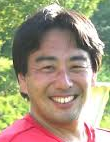
\includegraphics[height=\linewidth/2]{yugo.png}
    \caption{画像テスト}
    \label{fig:YUGO}
  \end{figure}
  \par


\section{先行研究}
  リモートセンシング技術による斜面崩壊・浸水領域検出に関する研究を以下に示す。
  
% \subsection{衛星画像を用いた斜面崩壊領域検出}
  % 江口ら\cite{art01}は地震と豪雨災害後の人工衛星画像を用いて斜面崩壊領域を検出する手法を提案している。この手法では人工衛星画像を土砂領域、植生領域、水領域に分類し、国土地理院提供のDEMデータにより斜面でない領域を除去することによって斜面崩壊領域を検出している。この手法では広範囲の解析が可能であり、衛星画像特有の指標にて容易に土地被覆分類ができるという利点がある。しかし、衛星画像は解像度が低く、条件によっては画像自体が取得できない可能性があり、斜面上の道路等の人工物を誤検出するという問題もある。

\subsection{ヘリコプター空撮画像を用いた斜面崩壊領域検出}
  中山ら\cite{art02}は地震災害後のヘリコプター空撮画像を用いて斜面崩壊領域を検出する手法を提案している。この手法ではL*a*b*色空間\cite{}にて土砂領域を検出し、テクスチャ特徴の一つである異質度\cite{}とDEMデータにて道路や平地を除去している。この手法では解像度の高さを利用した異質度にて人工物を除去することができるという利点がある。しかし,位置情報を含み,直下視点である衛星画像と比べ、DEMとの位置合わせの際に生じるずれにより精度が低下するという問題がある.

\subsection{ヘリコプター空撮画像を用いた浸水領域検出}
  雨宮ら\cite{art03}は豪雨災害後のヘリコプター空撮画像を用いて浸水領域を検出する手法を提案している。この手法でエッジ抽出率\cite{}と異質度を用いて、エッジ抽出率と異質度が低い領域を浸水領域として検出している。この手法では建物データと形状特徴にて建物領域を除去しすることができるという利点がある。しかし、この手法は都市部での検出を想定しており、山間部では建物データの位置合わせが難しく建物除去の精度が低下するという問題がある。


\section{本研究の目的} 
  以上の背景と先行研究を踏まえ、本研究では災害時の新たな観測手段としてドローンの活用を考える。本研究では建物データやDEMデータなどの補助データを用いること無く建物などの誤検出を抑え、災害後の高解像度ドローン空撮画像のみから斜面崩壊・浸水領域を検出する手法を提案する。また、衛星画像やヘリコプター空撮画像が使用不可能な場合の代替手段としてドローンの活用を考えるため、先行研究と同等の精度で災害領域を検出することを目的とする。


\section{本論文の構成}
  \label{sec:本論文の構成}
  本論文の構成を以下に示す. \par
  第1章では本研究の背景,先行研究,及び目的について述べた.\par
  第2章では本研究の提案手法について述べる.\par
  第3章では実験方法及び実験結果について述べる.\par
  第4章ではまとめとして結論及び今後の課題について述べる.

\end{document}
